\subsection{Experiments 4--7: Temporal Forecasting}

% Experiment 4 - GlobalPlasticsProduction

\begin{figure}[H]
	\centering
	\subfloat[Theil-Sen regression.]{
		\includegraphics[width=0.45\textwidth]{figures/global_forecasting_theil-sen_regression.png}
	}
	\hfill
	\subfloat[Ridge regression.]{
		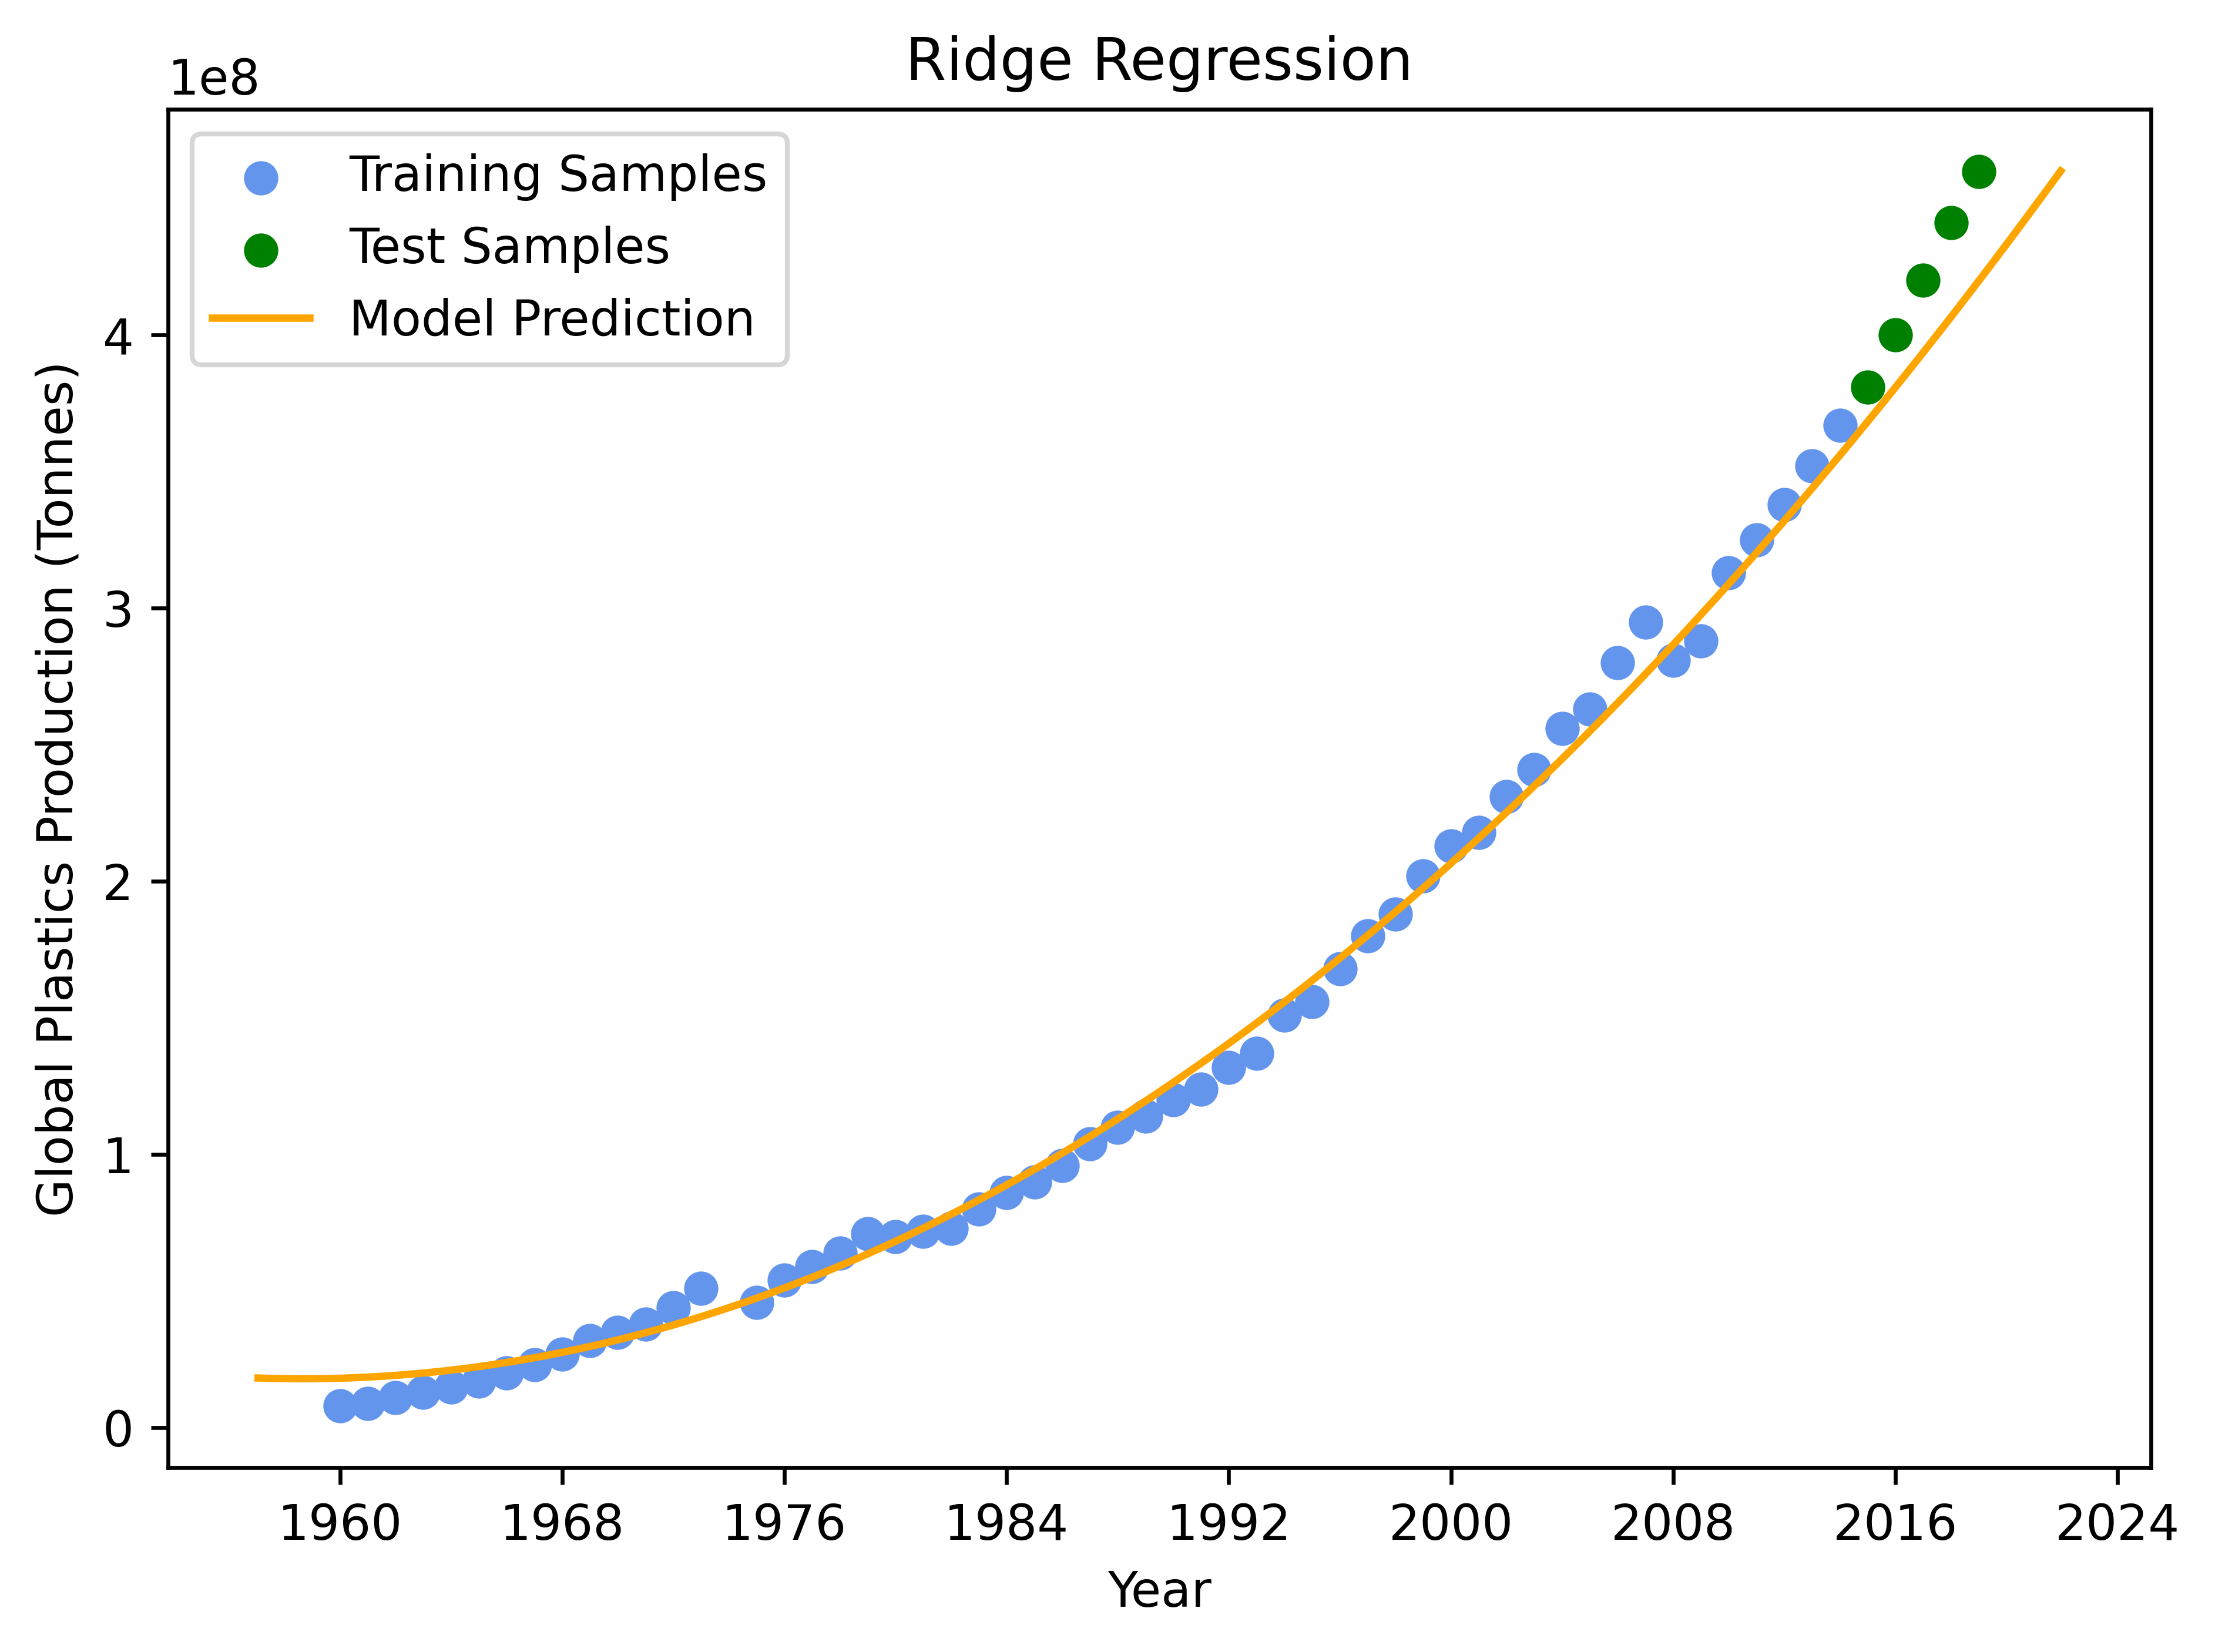
\includegraphics[width=0.45\textwidth]{figures/global_forecasting_ridge_regression.png}
	}

	\vspace{0.5cm}

	\subfloat[Gaussian process regression.]{
		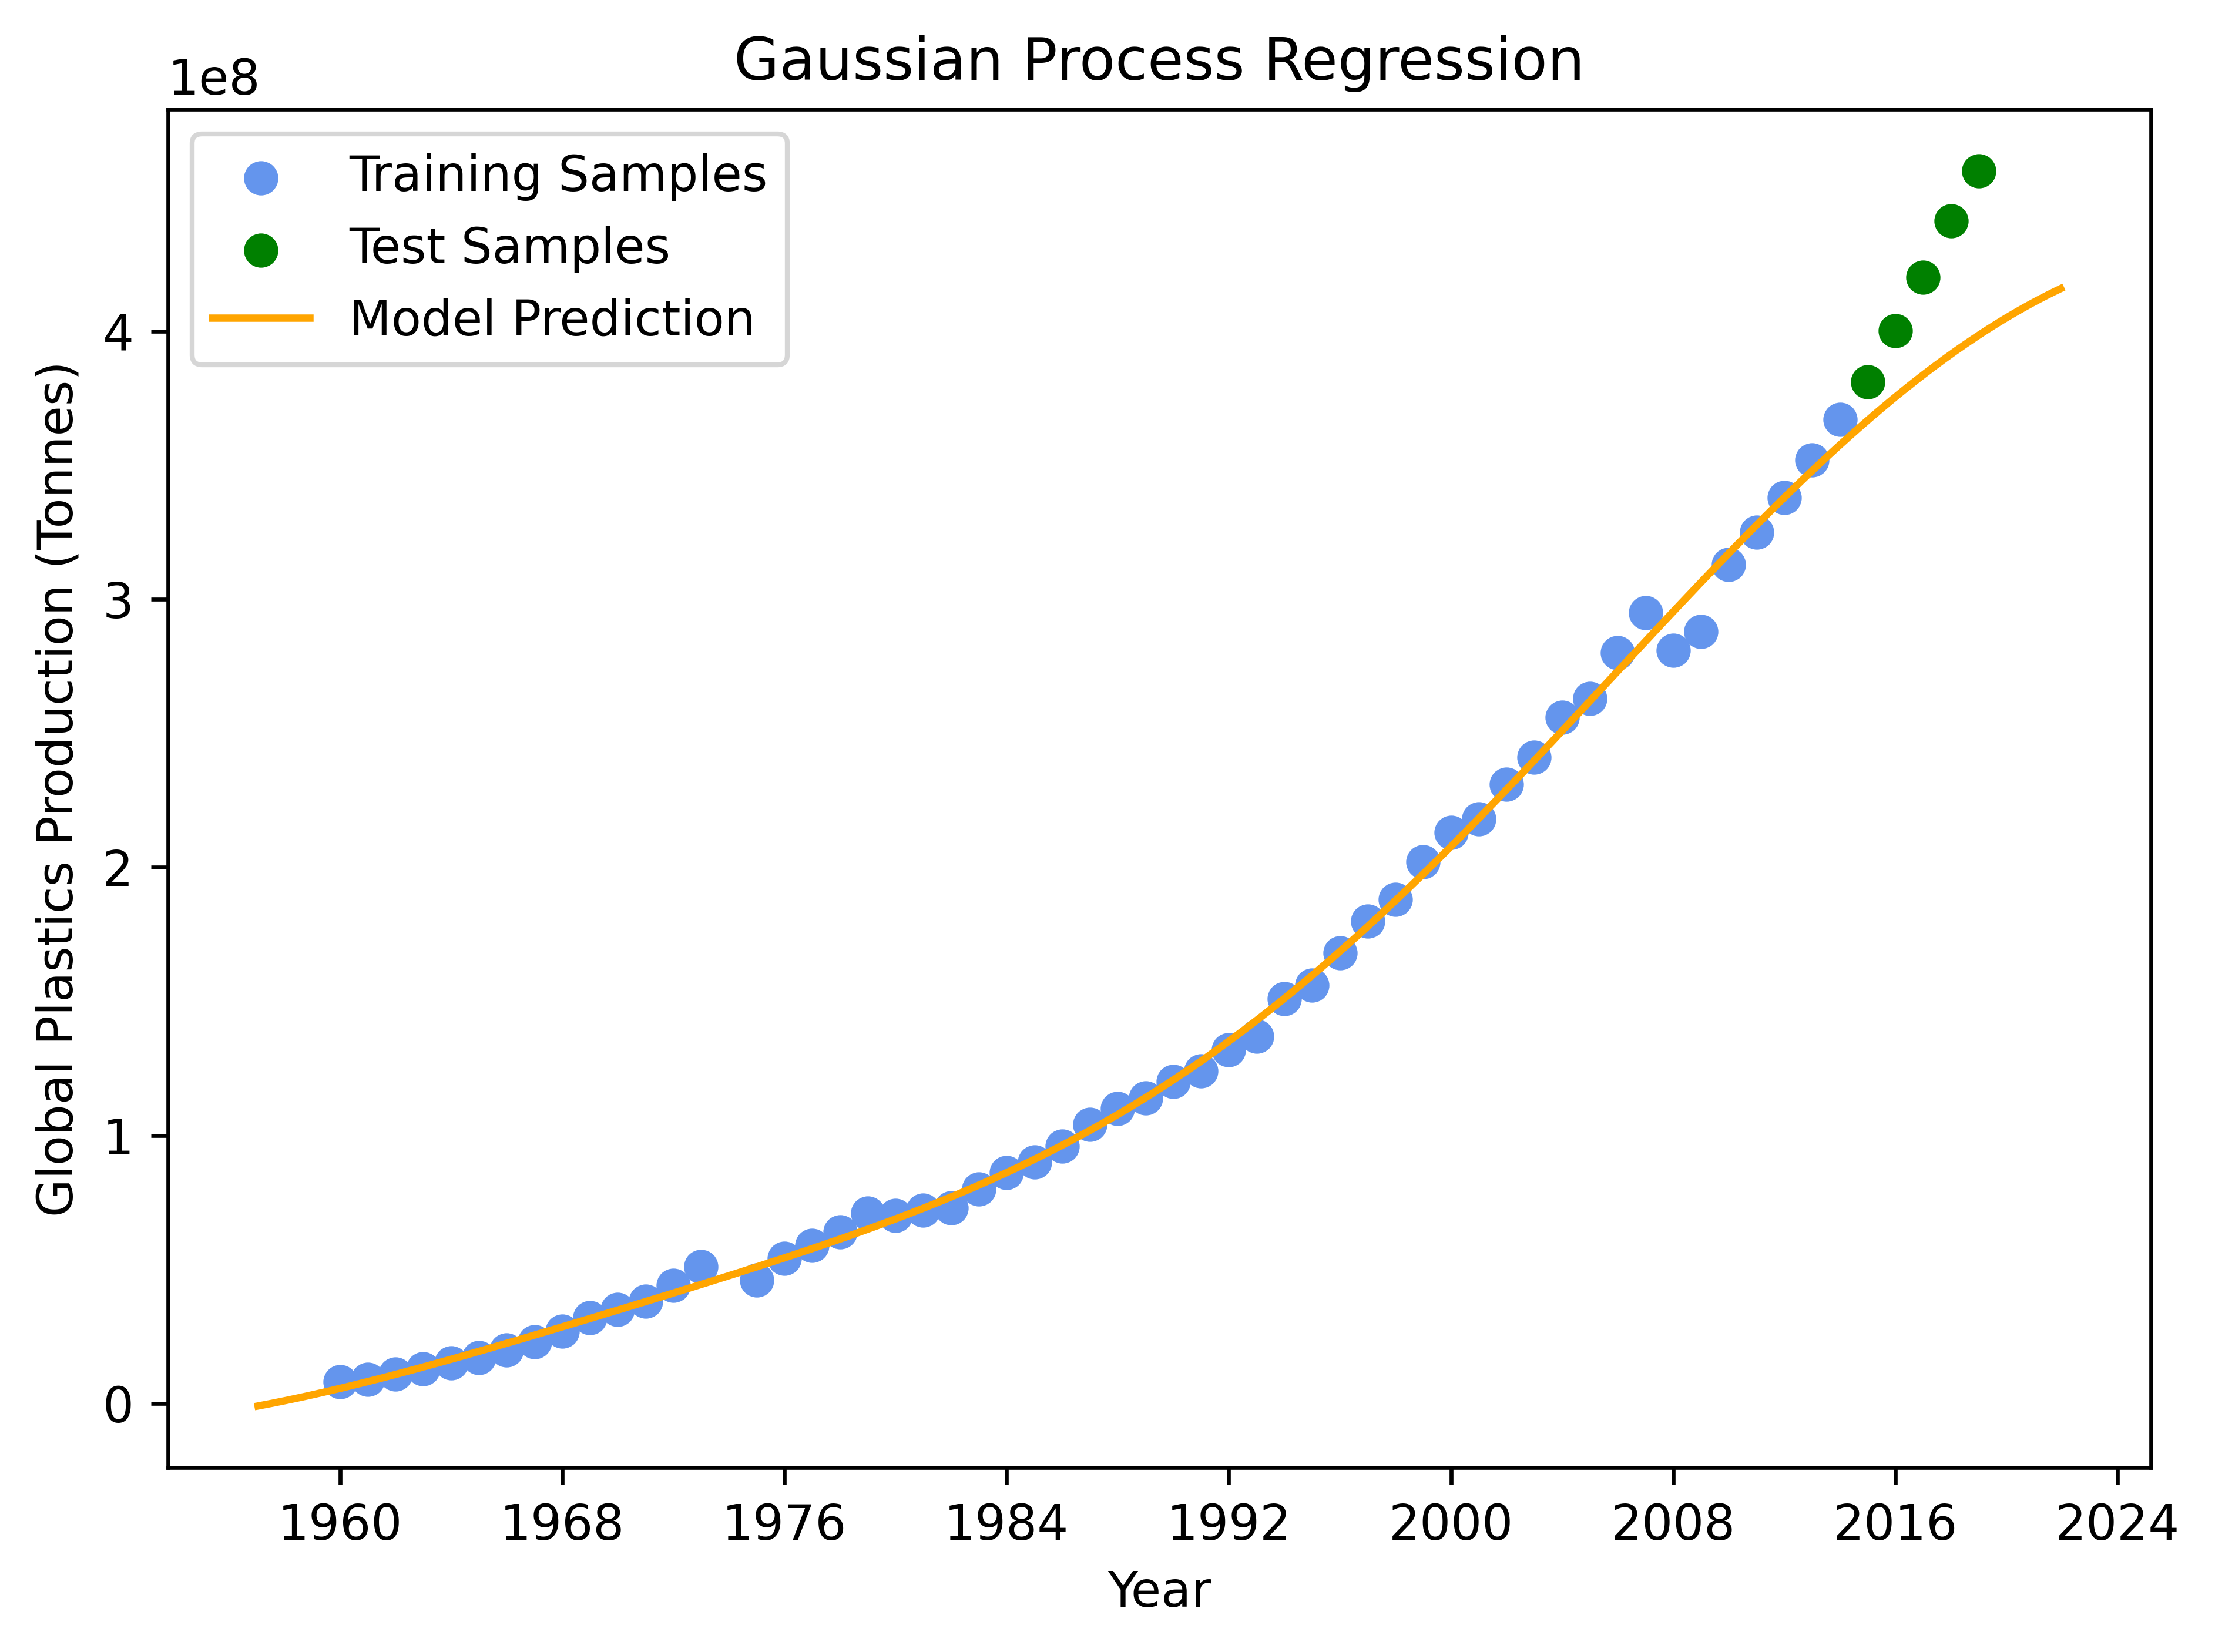
\includegraphics[width=0.45\textwidth]{figures/global_forecasting_gpr.png}
	}
	\subfloat[Support vector regression.]{
		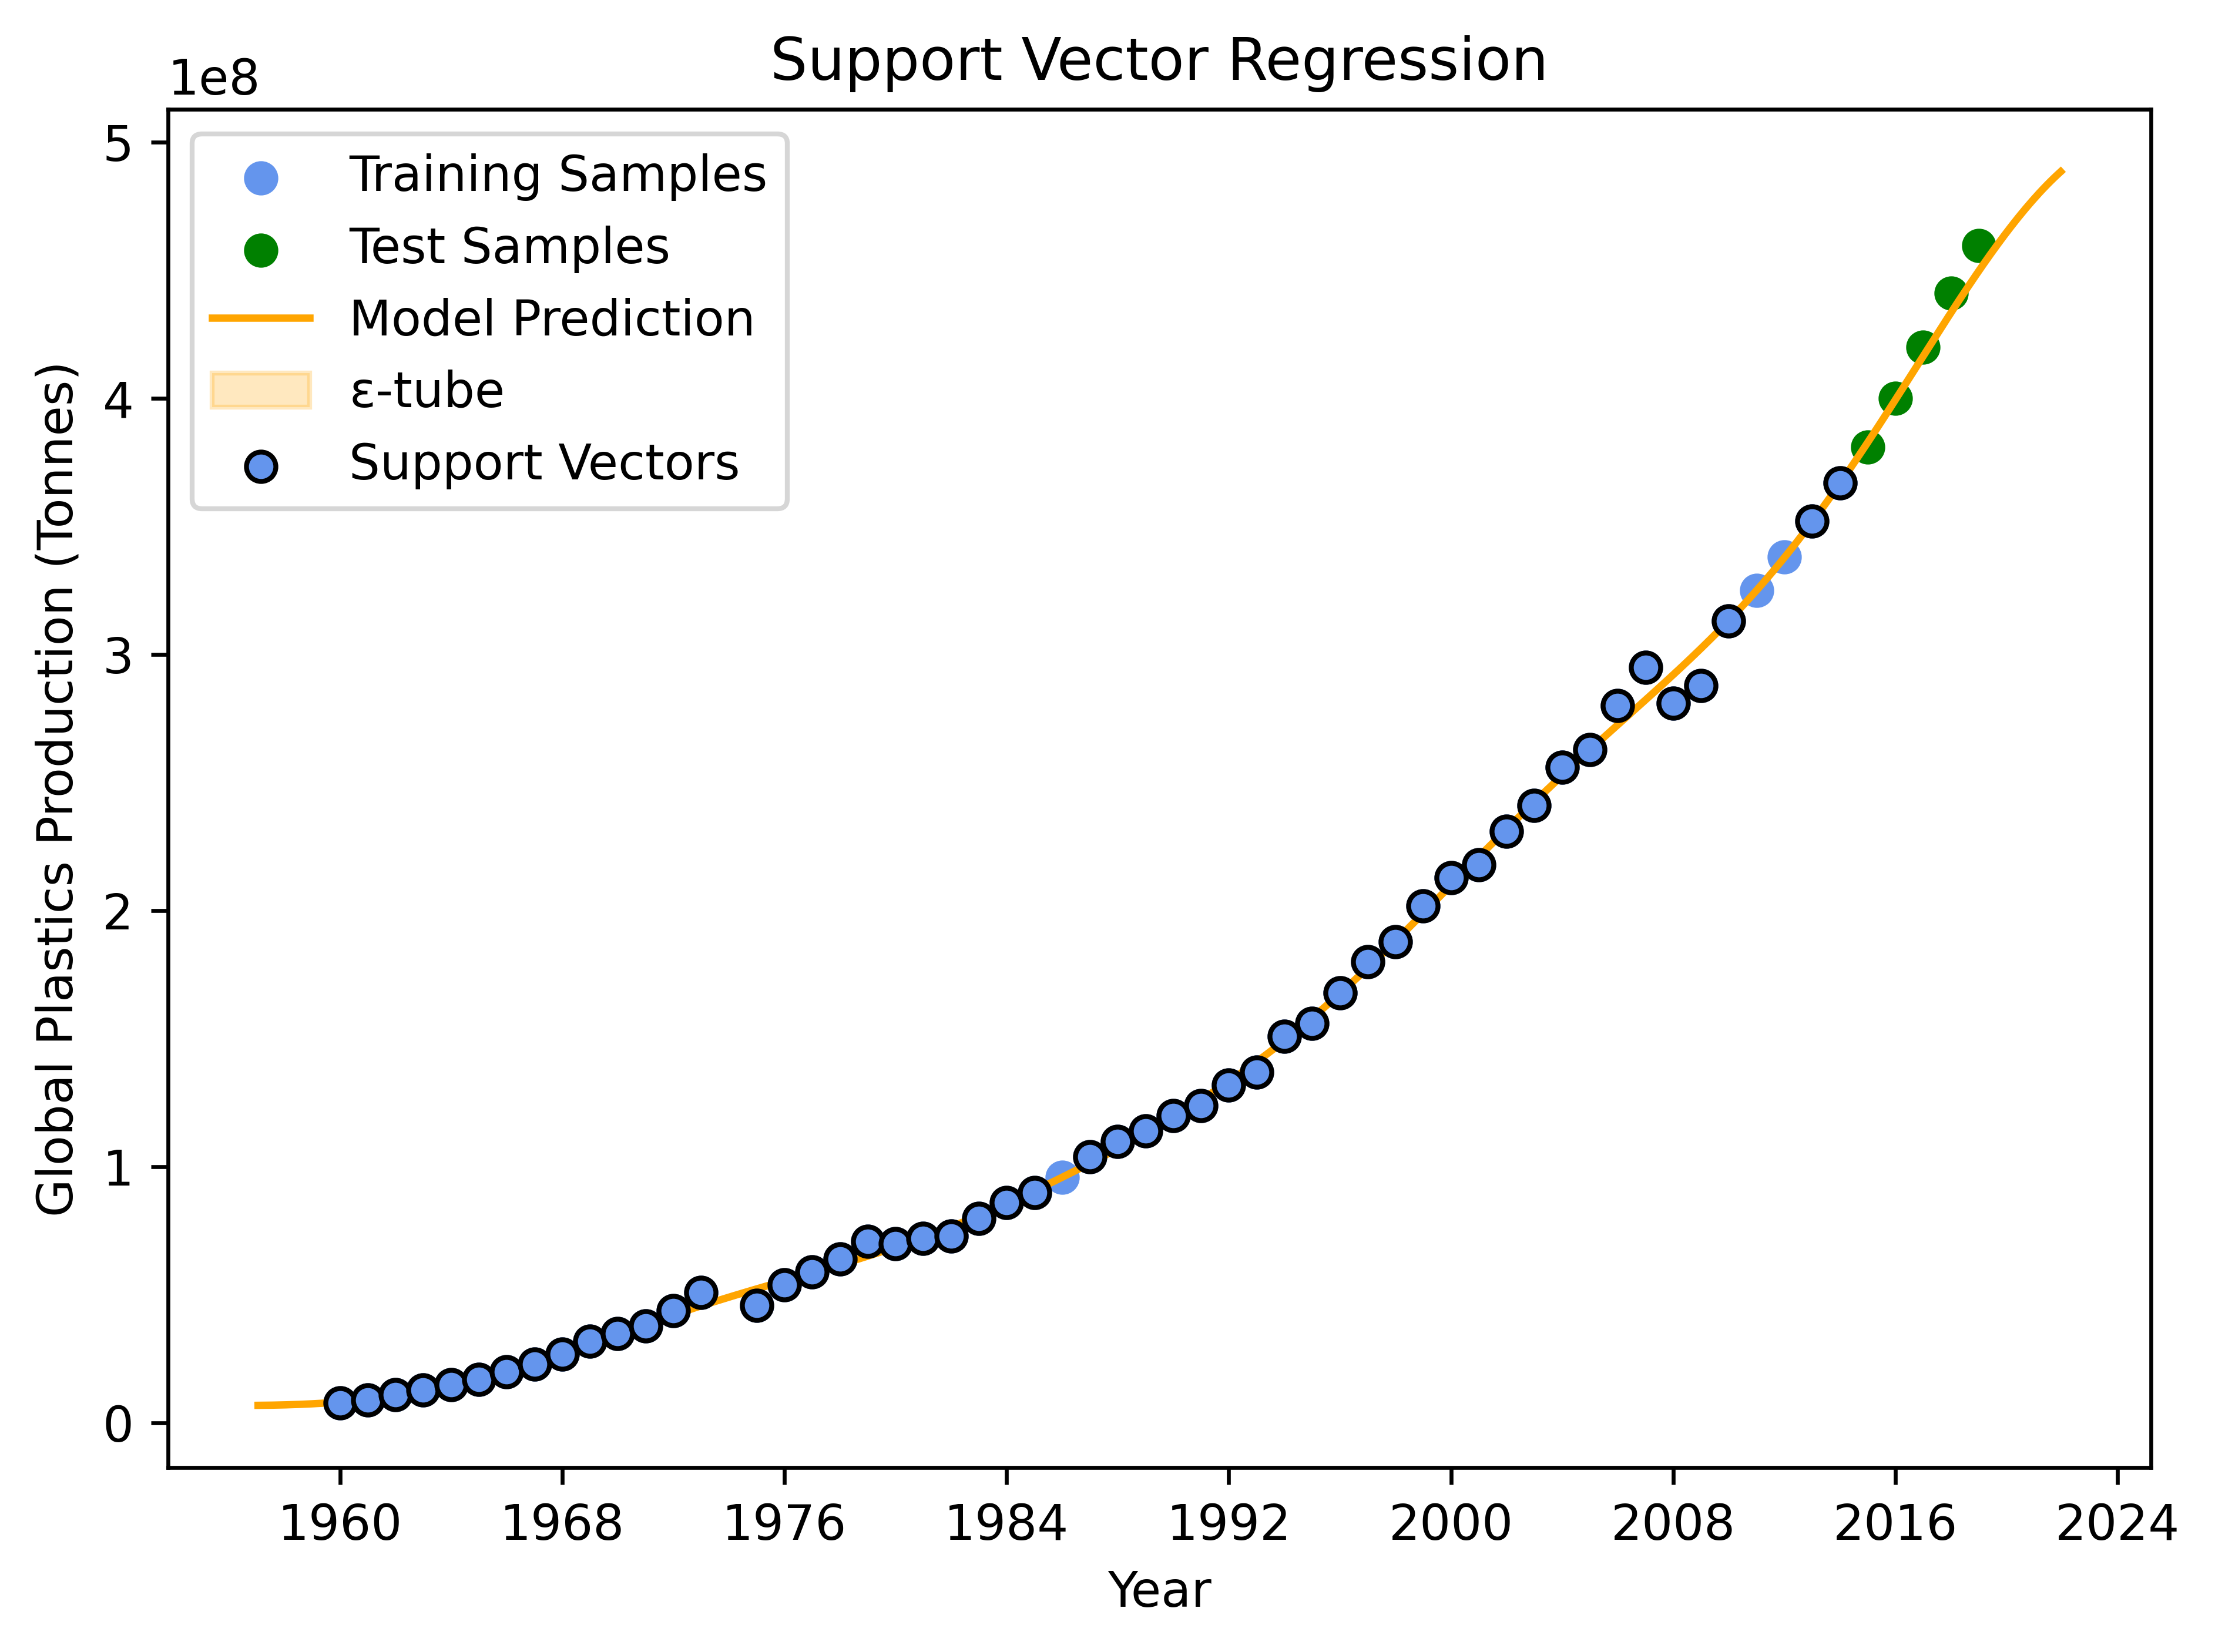
\includegraphics[width=0.45\textwidth]{figures/global_forecasting_svr.png}
	}

	\caption{Forecasts of global plastic production produced by four representative regression models.}
	\label{fig:global_forecasting_plots}
\end{figure}

\begin{table}[!ht]
	\centering
	\caption{\centering Temporal forecasting performance for global plastic production with grid search hyperparameter tuning.}
	\begin{tabular}{@{}lccccc@{}}
		\toprule
		\textbf{Experiment}                          & \textbf{MAE}                   & \textbf{RMSE}                  & $\mathbf{R^2}$     & \textbf{WAPE}       & \textbf{MAPE}       \\
		\midrule
		Naive Persistence                            & \(5.338 \times 10^7\)          & \(6.031 \times 10^7\)          & -3.615             & 12.70\%             & 12.31\%             \\
		Drift Baseline                               & \(3.344 \times 10^7\)          & \(3.830 \times 10^7\)          & -0.861             & 7.95\%              & 7.69\%              \\
		Exponential Smoothing                        & \(1.792 \times 10^7\)          & \(2.103 \times 10^7\)          & 0.439              & 4.26\%              & 4.10\%              \\
		Ridge Regression                             & \(3.261 \times 10^7\)          & \(3.421 \times 10^7\)          & -0.484             & 7.76\%              & 7.63\%              \\
		Gaussian Process Regression                  & \(3.722 \times 10^7\)          & \(4.086 \times 10^7\)          & -1.118             & 8.85\%              & 8.63\%              \\
		\textbf{Support Vector Regression}           & \(\mathbf{7.921 \times 10^6}\) & \(\mathbf{9.942 \times 10^6}\) & \(\mathbf{0.875}\) & \(\mathbf{1.88}\)\% & \(\mathbf{1.80}\)\% \\
		Support Vector Regression\textsuperscript{*} & \(2.590 \times 10^7\)          & \(2.806 \times 10^7\)          & 0.001              & 6.16\%              & 6.02\%              \\
		Theil-Sen Regression                         & \(1.111 \times 10^7\)          & \(1.365 \times 10^7\)          & 0.764              & 2.64\%              & 2.53\%              \\
		ARIMA Regression                             & \(2.103 \times 10^7\)          & \(2.477 \times 10^7\)          & 0.222              & 5.00\%              & 4.81\%              \\
		\hline
	\end{tabular}
	\label{tab:global_forecasting_grid_search_metric_table}
\end{table}

\begin{table}[!ht]
	\centering
	\caption{\centering Temporal forecasting performance for global plastic production with random search hyperparameter tuning.}
	\begin{tabular}{@{}lccccc@{}}
		\toprule
		\textbf{Experiment}                          & \textbf{MAE}                   & \textbf{RMSE}                  & $\mathbf{R^2}$     & \textbf{WAPE}       & \textbf{MAPE}       \\
		\midrule
		Naive Persistence                            & \(5.338 \times 10^7\)          & \(6.031 \times 10^7\)          & -3.615             & 12.70\%             & 12.31\%             \\
		Drift Baseline                               & \(3.344 \times 10^7\)          & \(3.830 \times 10^7\)          & -0.861             & 7.95\%              & 7.69\%              \\
		Exponential Smoothing                        & \(1.792 \times 10^7\)          & \(2.103 \times 10^7\)          & 0.439              & 4.26\%              & 4.10\%              \\
		Ridge Regression                             & \(2.657 \times 10^7\)          & \(2.834 \times 10^7\)          & -0.019             & 6.32\%              & 6.19\%              \\
		Gaussian Process Regression                  & \(3.722 \times 10^7\)          & \(4.086 \times 10^7\)          & -1.118             & 8.85\%              & 8.63\%              \\
		\textbf{Support Vector Regression}           & \(\mathbf{4.709 \times 10^6}\) & \(\mathbf{5.913 \times 10^6}\) & \(\mathbf{0.956}\) & \(\mathbf{1.12}\)\% & \(\mathbf{1.07}\)\% \\
		Support Vector Regression\textsuperscript{*} & \(2.503 \times 10^7\)          & \(2.727 \times 10^7\)          & 0.057              & 5.95\%              & 5.81\%              \\
		Theil-Sen Regression                         & \(1.111 \times 10^7\)          & \(1.365 \times 10^7\)          & 0.764              & 2.64\%              & 2.53\%              \\
		ARIMA Regression                             & \(2.103 \times 10^7\)          & \(2.477 \times 10^7\)          & 0.222              & 5.00\%              & 4.81\%              \\
		\hline
	\end{tabular}
	\label{tab:global_forecasting_random_search_metric_table}
\end{table}

% Table~\ref{tab:forecasting_results_grid_search} and Table~\ref{tab:forecasting_results_random_search} show that SVR achieved the best overall performance among all evaluated methods. In the random search tuning setting, SVR obtained the lowest MAE, RMSE, WAPE, and MAPE, and the highest \(R^2\) value. In the grid search tuning setting, SVR is also the best performing method, although it was slightly weaker than in the former setting. These results indicate that SVR was the most effective model for capturing the temporal trend in global plastic production. Figure~\ref{fig:global_forecasting_plots} visually confirms the superior performance of SVR, as its forecasted test values closely follow the actual test values, while the other methods show larger deviations.

Table~\ref{tab:global_forecasting_grid_search_metric_table} and Table~\ref{tab:global_forecasting_random_search_metric_table} indicate that SVR achieved the best overall performance among all evaluated methods. Under the random search tuning setting, SVR attained the lowest MAE, RMSE, WAPE, and MAPE, as well as the highest \(R^2\) value. Under the grid search setting, SVR also remained the top-performing method, although its performance was slightly inferior to that of the random search setting.

These results suggest that SVR is the most effective model for capturing the temporal trend in global plastic production. Figure~\ref{fig:global_forecasting_plots} further supports this conclusion, as the SVR forecasts closely follow the actual test values, whereas the other methods exhibit larger deviations.

\begin{table}[!ht]
	\centering
	\caption{\centering Hyperparameter tuning time for tunable temporal forecasting models under grid search and random search.}
	\begin{tabular}{@{}lcc@{}}
		\toprule
		\textbf{Experiment}                          & \textbf{Grid Search (ms)} & \textbf{Random Search (ms)} \\
		\midrule
		Ridge Regression                             & 6331.585                  & 2985.758                    \\
		Gaussian Process Regression                  & 158576.799                & 133046.250                  \\
		Support Vector Regression                    & 4150.489                  & 3186.485                    \\
		Support Vector Regression\textsuperscript{*} & 61600.061                 & 2771.060                    \\
		\hline
	\end{tabular}
	\label{tab:forecasting_tuning_time}
\end{table}

% Table~\ref{tab:forecasting_results_grid_search} and Table~\ref{tab:forecasting_results_random_search} also show that for all the tunable models, random search always has equal to better performance than grid search. Moreover, Table~\ref{tab:forecasting_tuning_time} suggests that random search is more efficient than grid search in terms of hyperparameter tuning time in this experiment settings. Therefore, in the following experiments, we will only report the results of random search tuning for the tunable models.

Table~\ref{tab:global_forecasting_grid_search_metric_table} and Table~\ref{tab:global_forecasting_random_search_metric_table} also show that, for all tunable models, random search consistently achieves performance that is equal to or better than that of grid search. Furthermore, Table~\ref{tab:forecasting_tuning_time} indicates that random search is more efficient in terms of hyperparameter tuning time under the experimental settings considered. Therefore, in the subsequent experiments, we report only the results obtained using random search for the tunable models.

% Experiment 5 - YearPWG (Japan)

\begin{figure}[H]
	\centering
	\subfloat[Arima regression.]{
		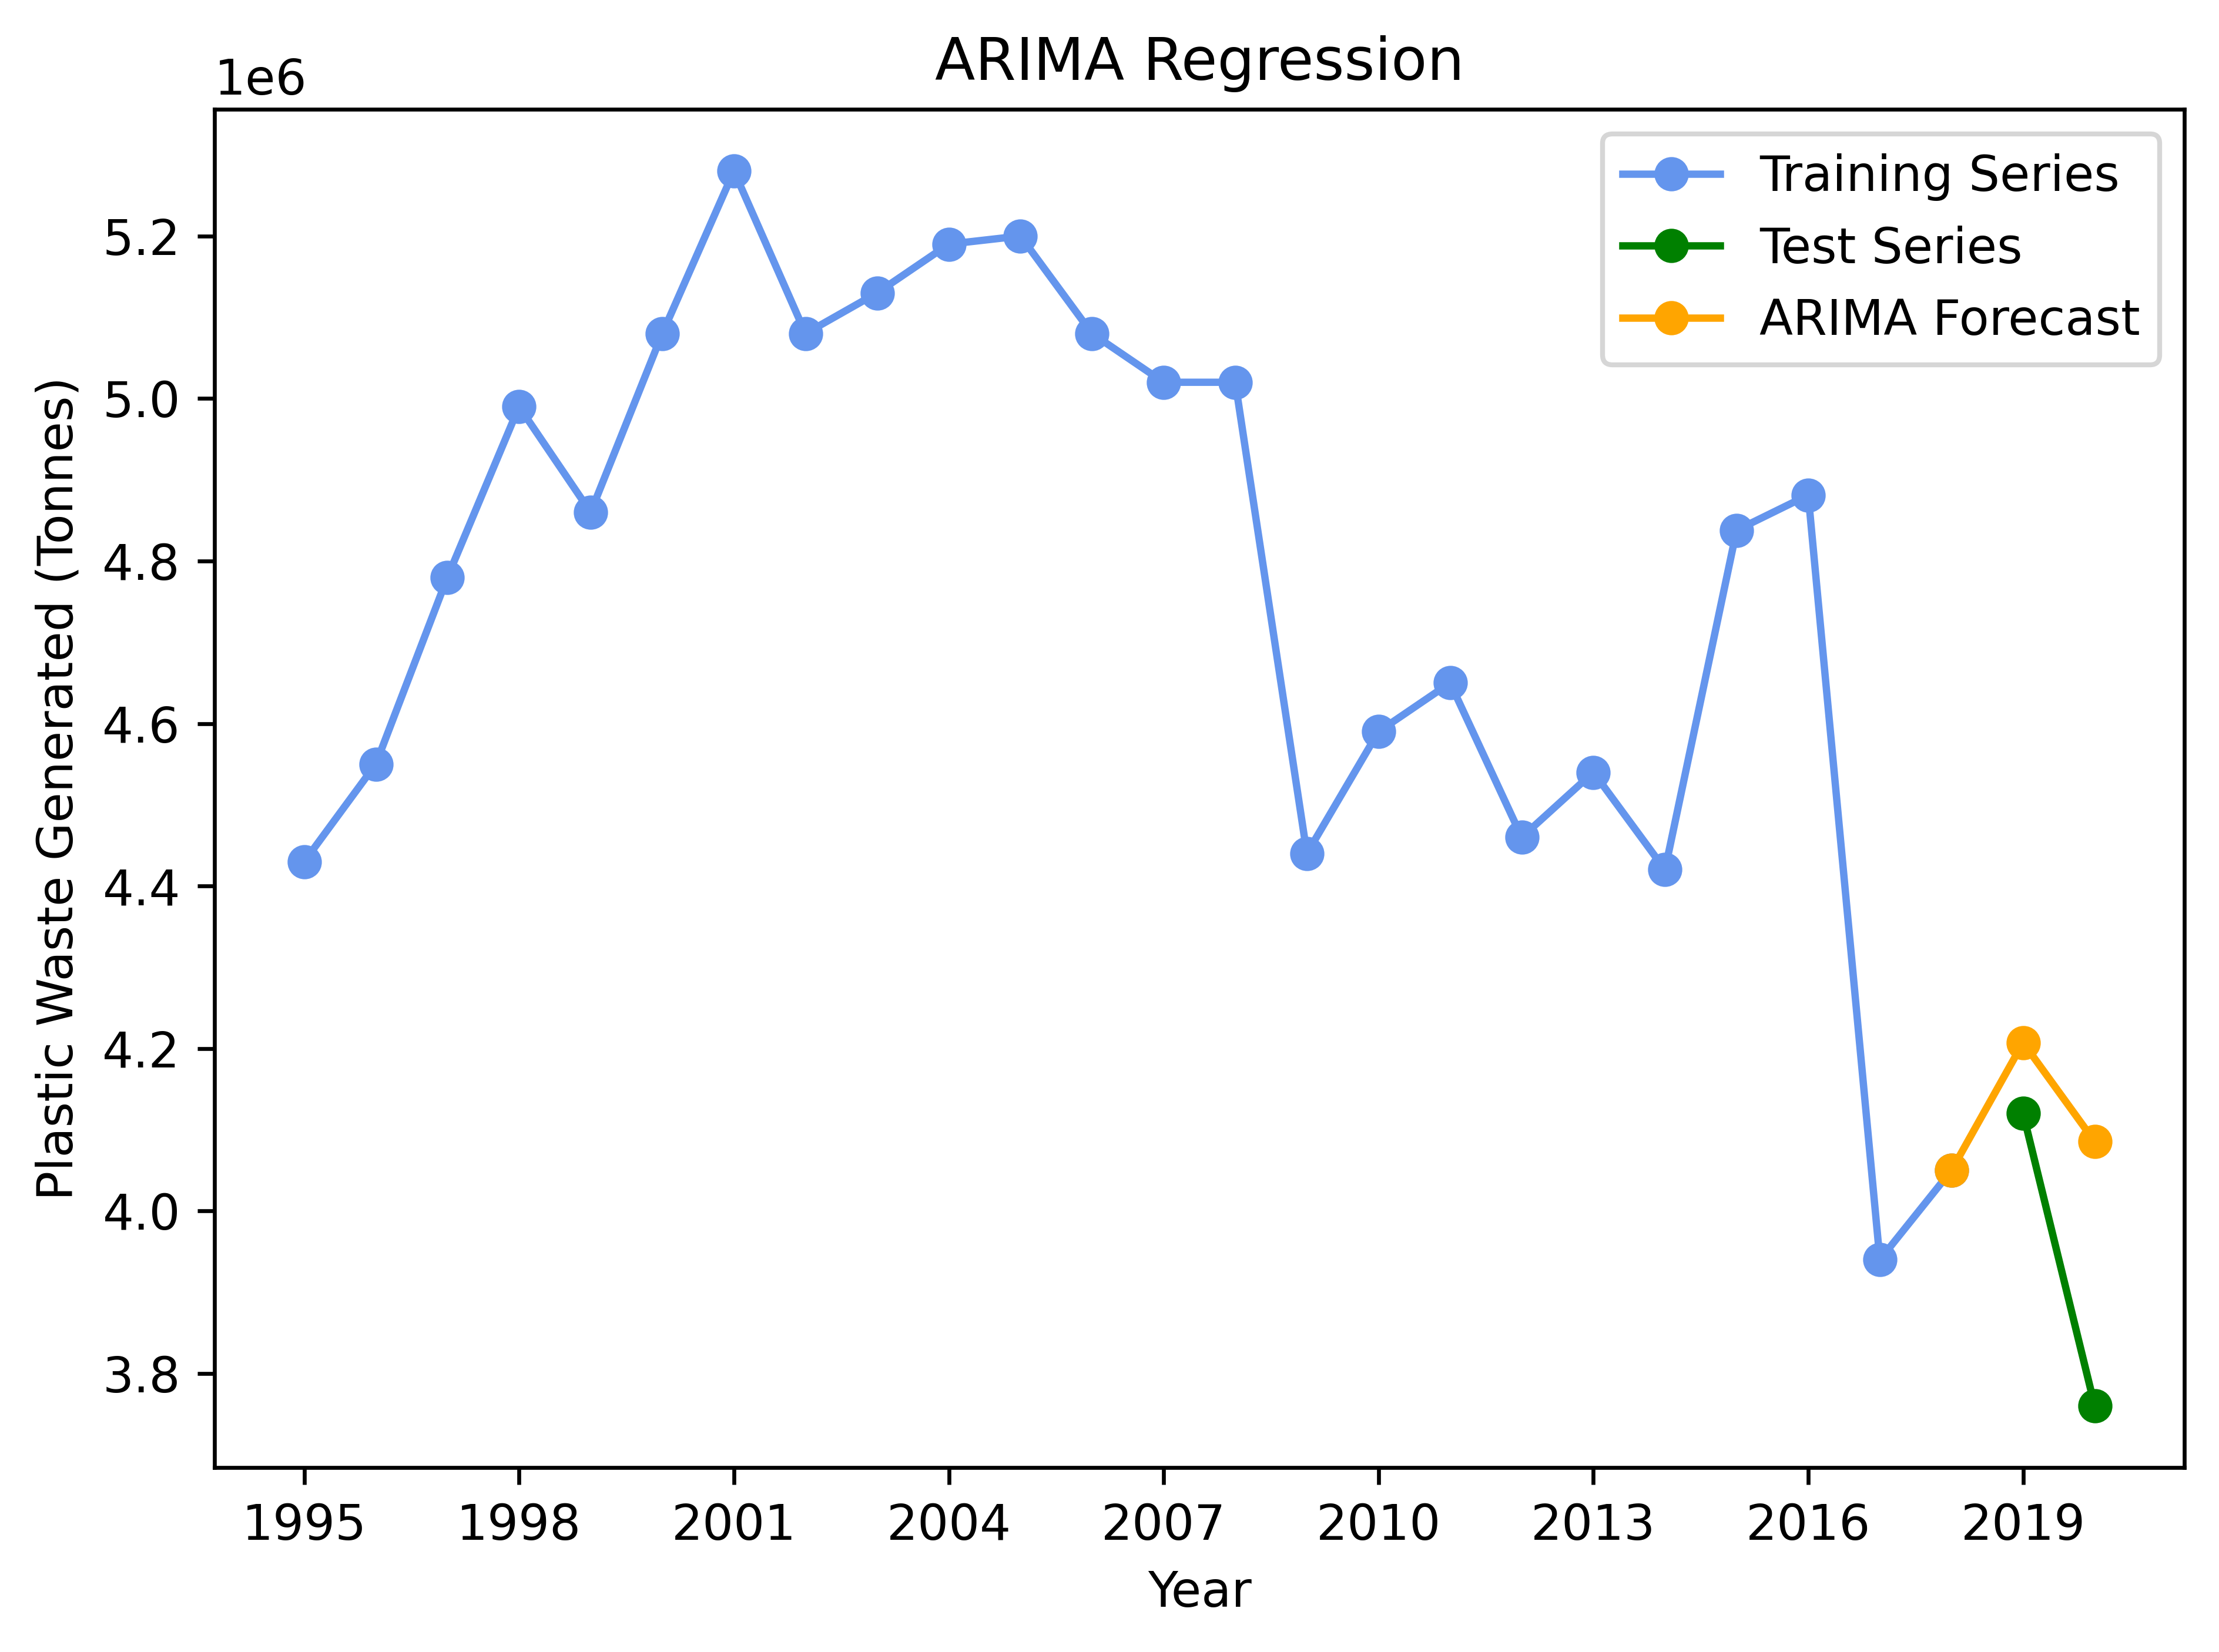
\includegraphics[width=0.45\textwidth]{figures/japan_pwg_forecasting_arima_regression.png}
	}
	\hfill
	\subfloat[Ridge regression.]{
		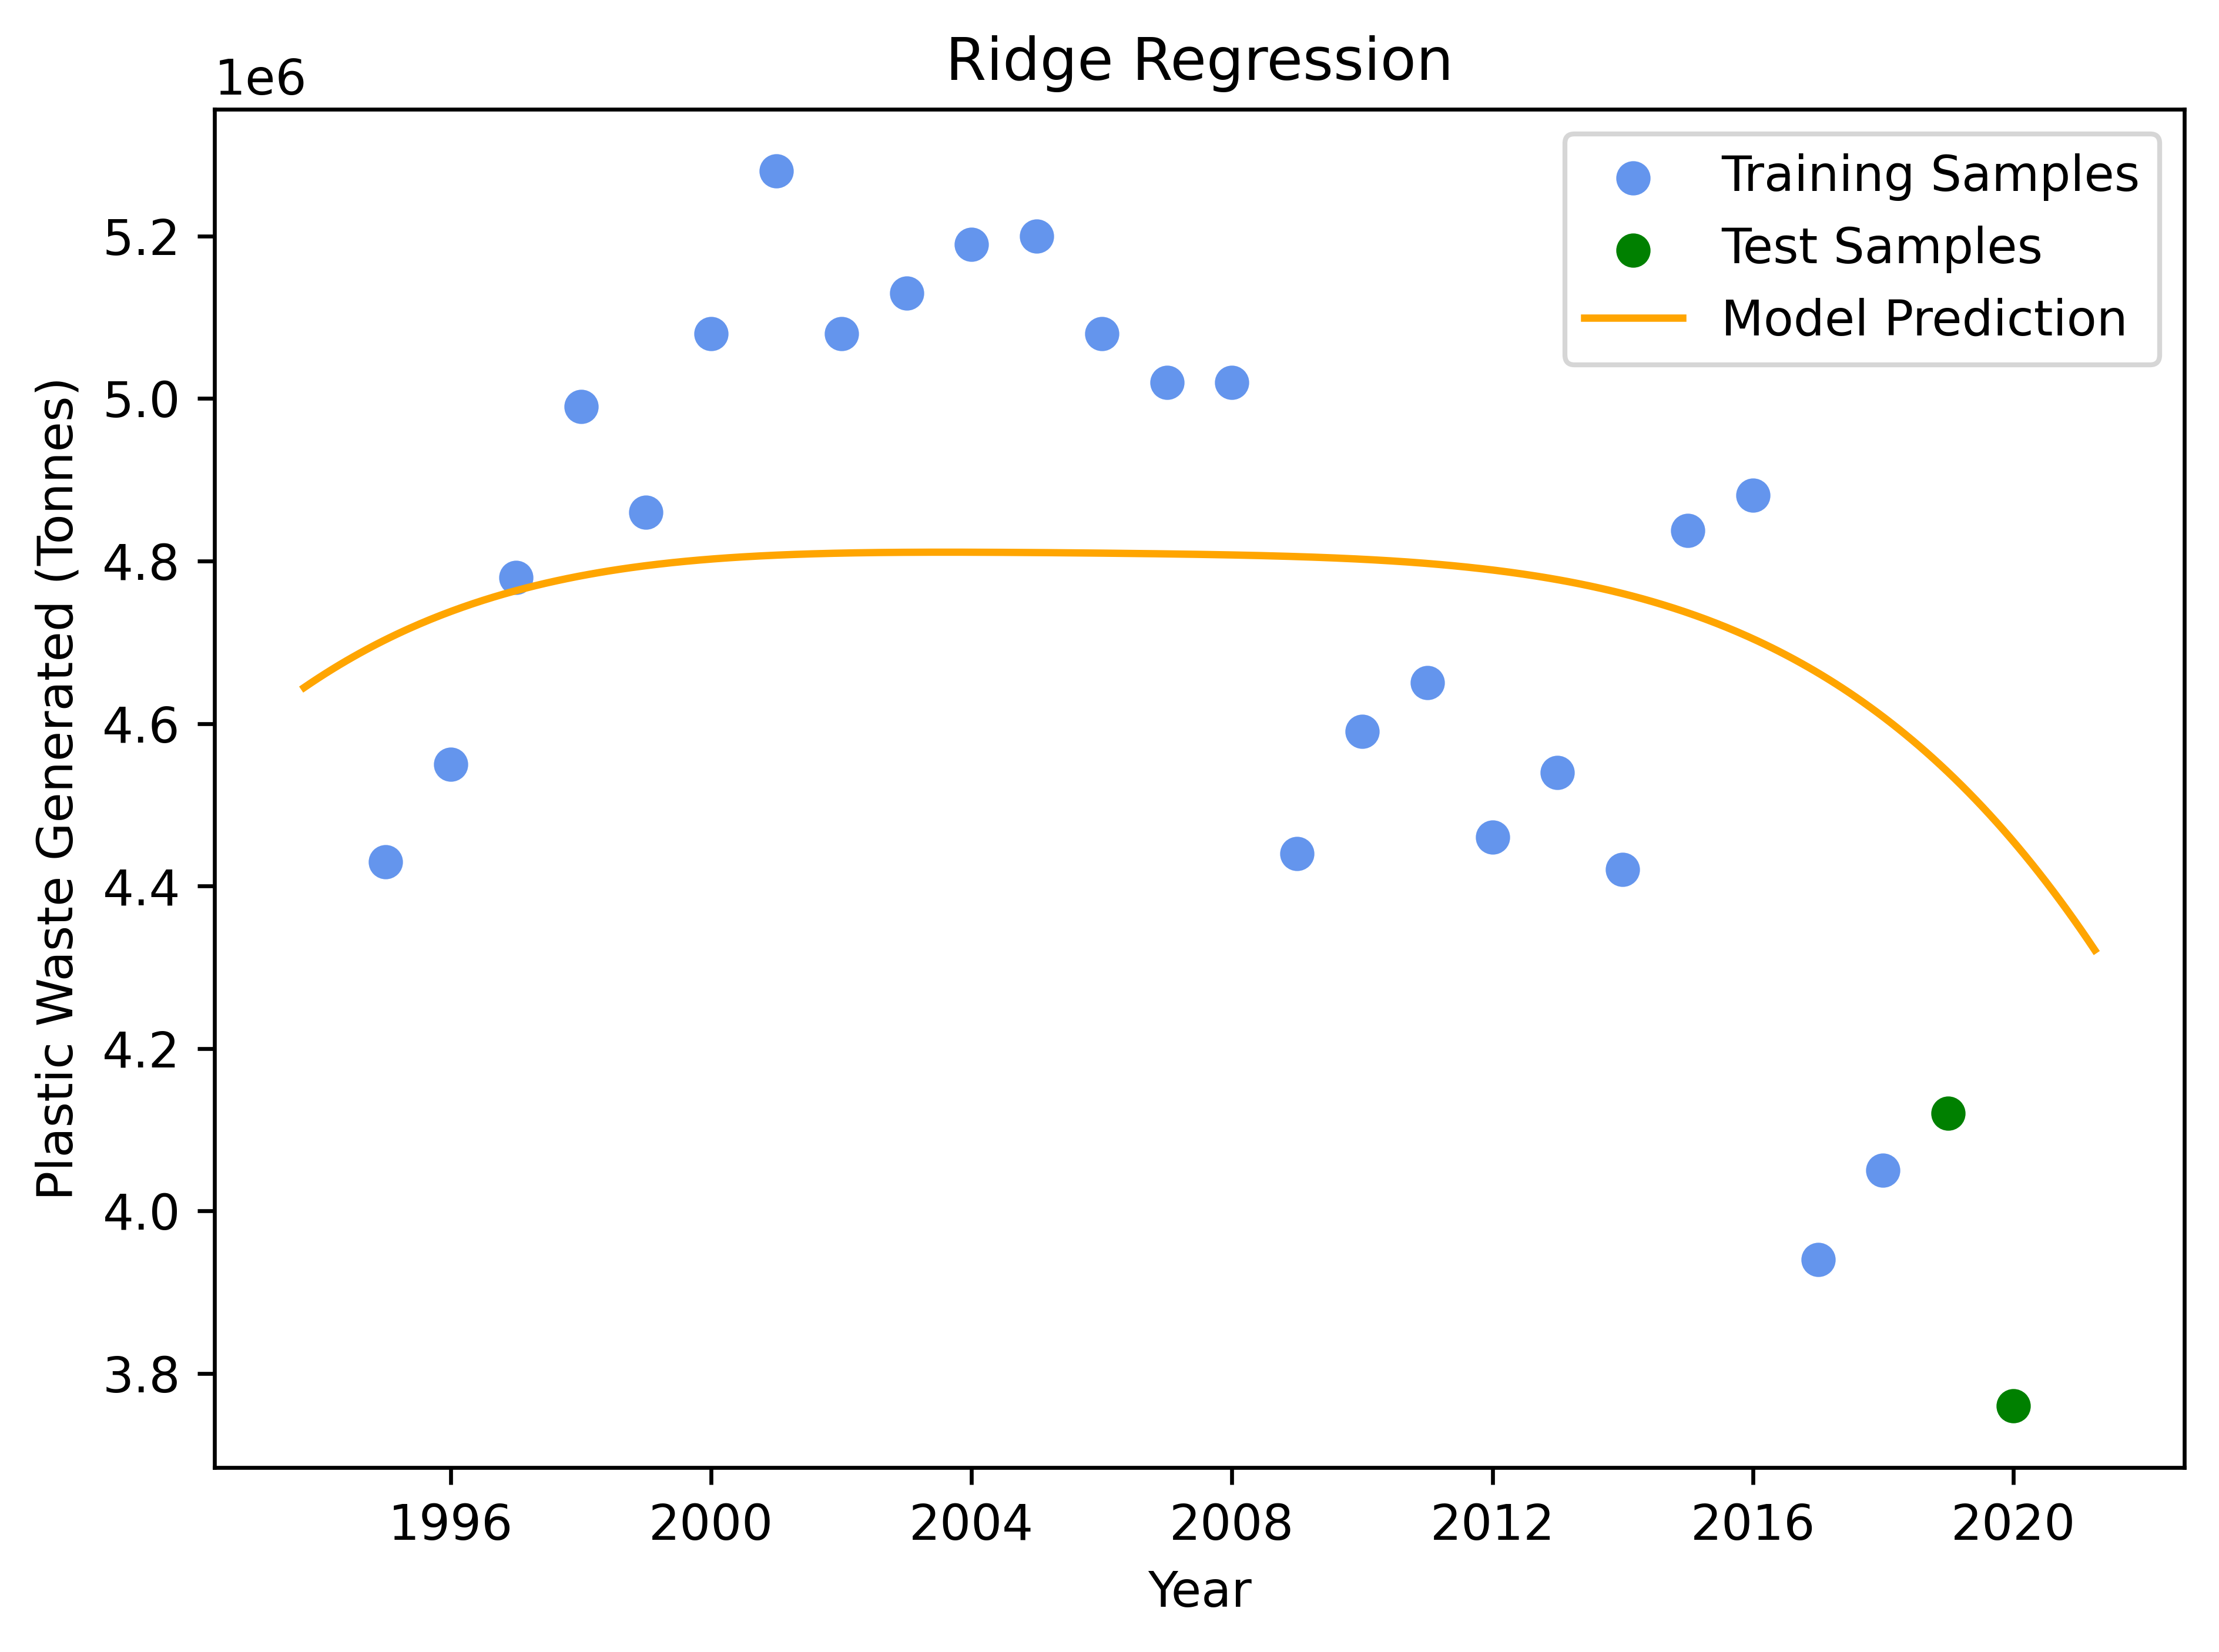
\includegraphics[width=0.45\textwidth]{figures/japan_pwg_forecasting_ridge_regression.png}
	}

	\vspace{0.5cm}

	\subfloat[Gaussian process regression.]{
		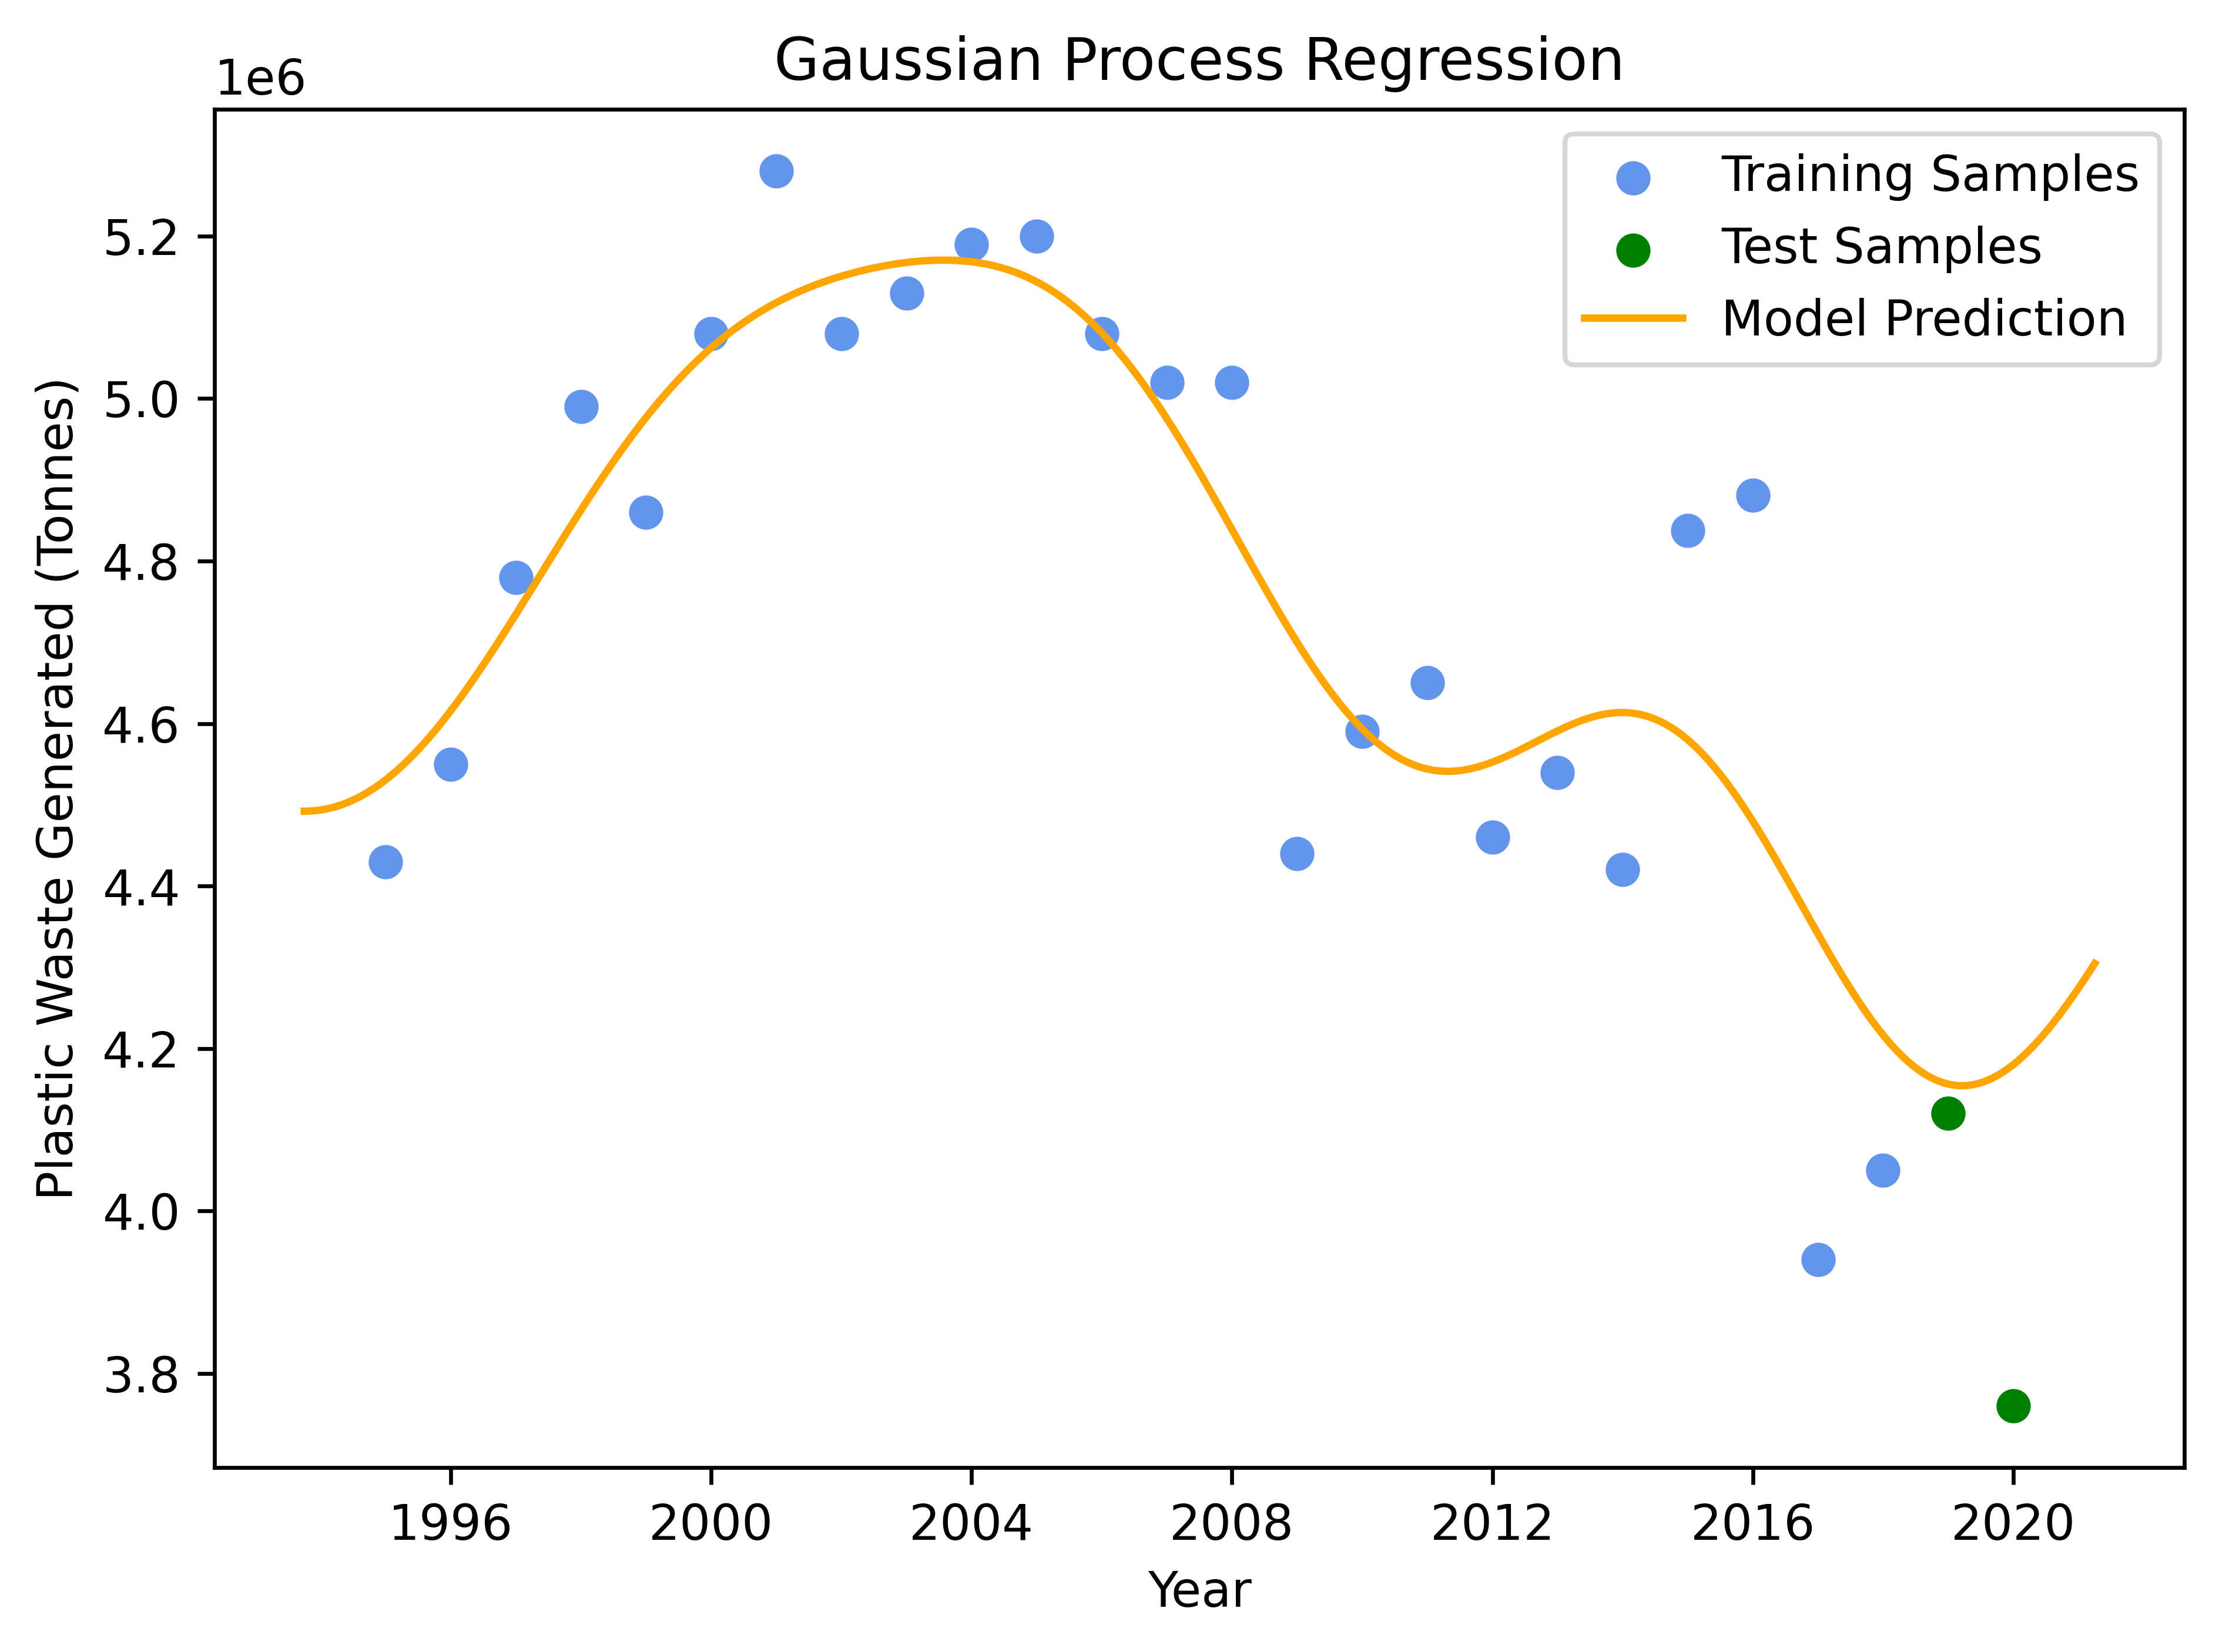
\includegraphics[width=0.45\textwidth]{figures/japan_pwg_forecasting_gpr.png}
	}
	\subfloat[Support vector regression.]{
		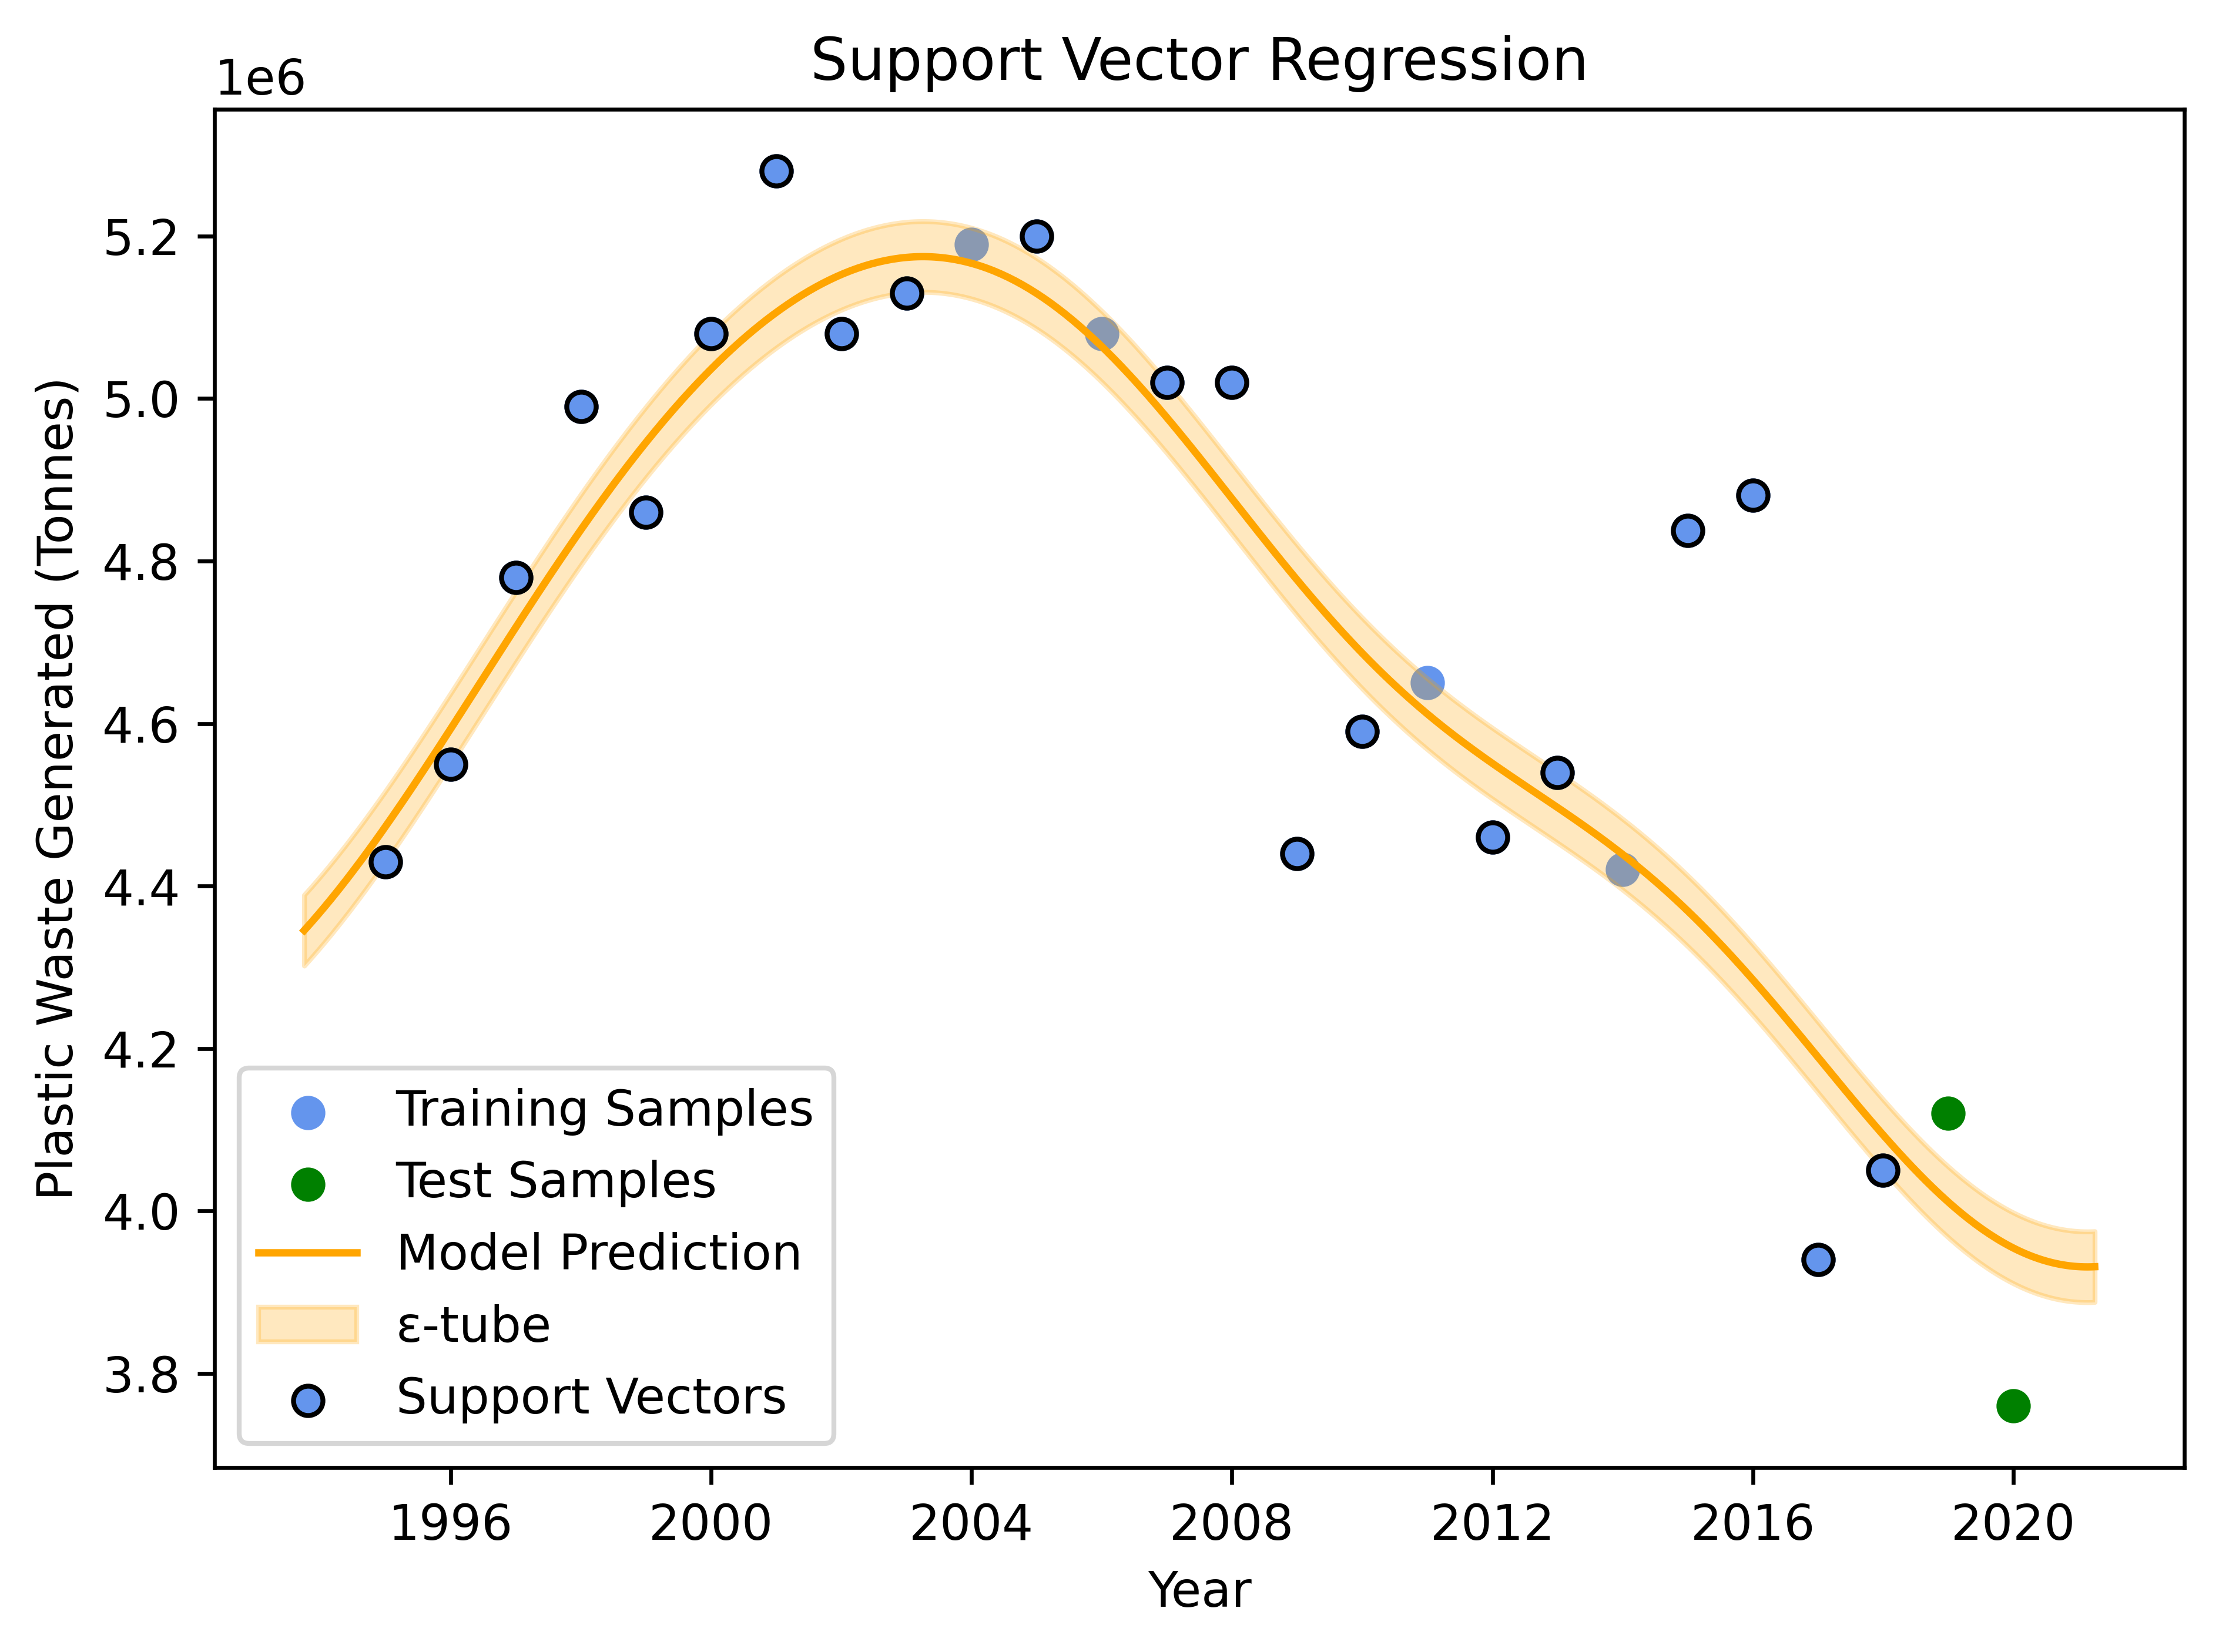
\includegraphics[width=0.45\textwidth]{figures/japan_pwg_forecasting_svr.png}
	}

	\caption{Forecasts of plastic waste generation in Japan by four representative regression models.}
	\label{fig:japan_pwg_forecasting_plots}
\end{figure}

% Experiment 6 - PWDrivers

\begin{table}[!ht]
	\centering
	\caption{\centering Temporal forecasting performance for global plastic production.}
	\begin{tabular}{@{}lccccc@{}}
		\toprule
		\textbf{Experiment}                           & \textbf{MAE}          & \textbf{RMSE}         & $\mathbf{R^2}$     & \textbf{WAPE}       & \textbf{MAPE}       \\
		\midrule
		Naive Persistence                             & \(1.800 \times 10^5\) & \(2.110 \times 10^5\) & -0.373             & 4.57\%              & 4.71\%              \\
		Drift Baseline                                & \(1.717 \times 10^5\) & \(1.917 \times 10^5\) & -0.134             & 4.36\%              & 4.47\%              \\
		Exponential Smoothing                         & \(1.379 \times 10^5\) & \(1.424 \times 10^5\) & \(\mathbf{0.374}\) & \(\mathbf{3.50}\)\% & \(\mathbf{3.55}\)\% \\
		Ridge Regression                              & \(5.573 \times 10^5\) & \(5.740 \times 10^5\) & -9.170             & 14.15\%             & 14.33\%             \\
		Gaussian Process Regression                   & \(2.282 \times 10^5\) & \(2.982 \times 10^5\) & -1.745             & 5.79\%              & 6.03\%              \\
		Support Vector Regression                     & \(1.516 \times 10^5\) & \(1.576 \times 10^5\) & 0.234              & 3.85\%              & 3.91\%              \\
		Support Vector Regression (with gamma tuning) & \(1.452 \times 10^5\) & \(1.839 \times 10^5\) & -0.044             & 3.69\%              & 3.82\%              \\
		Theil-Sen Regression                          & \(1.491 \times 10^5\) & \(2.002 \times 10^5\) & -0.236             & 3.78\%              & 3.95\%              \\
		ARIMA Regression                              & \(2.063 \times 10^5\) & \(2.382 \times 10^5\) & -0.752             & 5.24\%              & 5.39\%              \\
		\hline
	\end{tabular}
	\label{tab:japan_pwg_forecasting_metric_table}
\end{table}

% Experiment 7 - PWDrivers (Japan) & PWDrivers (Slovenia)
